\documentclass[tikz,border=5mm]{standalone}
\begin{document}

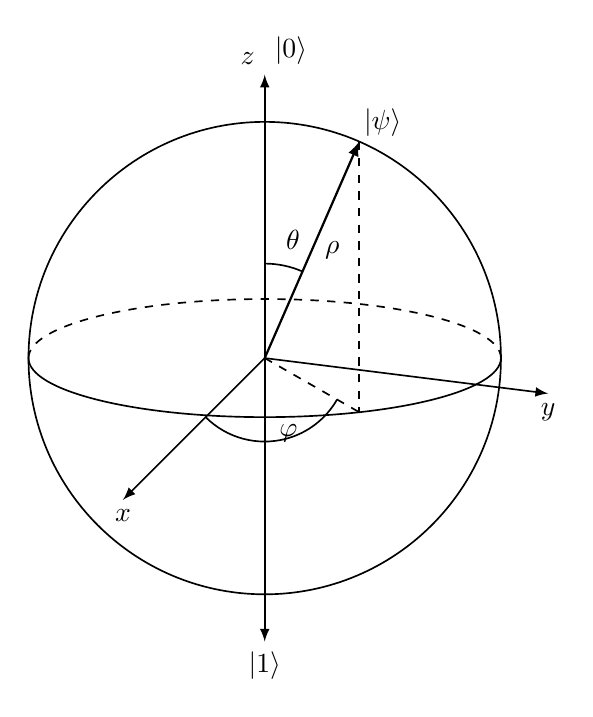
\begin{tikzpicture}[scale=3, >=latex, line width=0.6pt]

  % Define the sphere outline
  \draw (0,0) circle (1cm);

  % Draw the equator (solid in front, dashed in back)
  \draw (1,0) arc (0:-180:1cm and 0.25cm);
  \draw[dashed] (1,0) arc (0:180:1cm and 0.25cm);

  % Draw the Cartesian axes
  \draw[->] (0,0) -- (-0.6,-0.6) node[below] {$x$};
  \draw[->] (0,0) -- (1.2,-0.15) node[below] {$y$};
  \draw[->] (0,0) -- (0,1.2) node[above left] {$z$} node[above right] {$|0\rangle$};
  \draw[->] (0,0) -- (0,-1.2) node[below] {$|1\rangle$};

  % Define coordinates for the state vector and its projection
  % Calculated so the tip lies exactly on the sphere and projection on the equator
  \coordinate (P) at (0.4, 0.9165);
  \coordinate (Pproj) at (0.4, -0.229);

  % Draw dashed projection lines
  \draw[dashed] (P) -- (Pproj);
  \draw[dashed] (0,0) -- (Pproj);

  % Draw the state vector with \rho and |\psi> labels
  \draw[->, thick] (0,0) -- (P) node[midway, right=1pt] {$\rho$} node[above right=-2pt] {$|\psi\rangle$};

  % Draw the polar angle \theta
  \draw (0, 0.4) arc (90:66.4:0.4);
  \node at (0.12, 0.5) {$\theta$};

  % Draw the azimuthal angle \varphi (from x-axis to the projection line)
  \draw (-0.25, -0.25) arc (225:330.2:0.353);
  \node at (0.1, -0.32) {$\varphi$};

\end{tikzpicture}

\end{document}
